\section{Active vs. Passive Convention}
\label{sec:app:convention}
Misorientation quaternions are represented in the active sense\footnote{The passive convention is used in \cite{francisGeodesicOctonionMetric2019}}:
\begin{equation}
	q_m = {q_A}^{-1}q_B
\end{equation}
where $q_m$, $q_A$, and $q_B$ represent the misorientation quaternion, orientation quaternion of grain A in the sample frame, and orientation quaternion of grain B in the sample frame, respectively. The $^{-1}$ operator denotes a unit quaternion inverse (identical to conjugation of a unit quaternion). Quaternion multiplication is given by equation 23 of \cite{rowenhorstConsistentRepresentationsConversions2015}
\begin{equation}
	p q \equiv\left(p_{0} q_{0}-\mathbf{p} \cdot \mathbf{q}, q_{0} \mathbf{p}+p_{0} \mathbf{q}+P \mathbf{p} \times \mathbf{q}\right)
\end{equation}
where $q_0$ and $p_0$ are scalar components of the quaternions, and $\mathbf{q}$ and $\mathbf{p}$ are the vector components.

In this work, we use the convention that $P=1$ throughout the various operations in the \vfzorepo{} ($P \equiv $ \matlab{epsijk}) and highly encourage interested readers to refer to \citet{rowenhorstConsistentRepresentationsConversions2015} to understand the redefined versions of quaternion multiplication, quaternion rotation, nuances associated with use of active vs. passive conventions, etc. \Gls{bp} unit normals are expressed pointing away from grain A and in the reference frame of grain A (i.e. the outward-pointing normal convention).

\section{Detailed Barycentric Interpolation Method}
\label{sec:app:bary}
\renewcommand\thefigure{\thesection.\arabic{figure}} 
\setcounter{figure}{0}

We describe barycentric interpolation applied in the \gls{vfz} framework in more detail. This includes:
\begin{itemize}
	\item[1.] triangulation of a \gls{vfz} mesh (\cref{sec:app:bary:tri})
	\item[2.] finding intersections between arbitrary \glspl{vfzgbo} and the \gls{vfz} mesh (i.e. finding intersecting facets) (\cref{sec:app:bary:int})
	\item[3.] calculating interpolated values of an arbitrary \gls{vfzgbo} property using the intersecting facet (\cref{sec:app:bary-interp})
\end{itemize}

\subsection{Triangulating a \glsentrytitlecase{vfz}{long} Mesh}
\label{sec:app:bary:tri}

Creation of a simplicial mesh is necessary to perform barycentric interpolation. Due to the difficulty of visualizing a 7-sphere, we provide visual illustrations of the process as applied to lower-dimensional analogues. After \glspl{gbo} have been symmetrized into a \gls{vfz} (\cref{sec:methods:framework:vfz}), the triangulation process occurs by:
\begin{enumerate}
	\item[1.1] applying a \gls{svd} transformation to remove the U(1)-symmetry degeneracy inherent in the \gls{vfzgbo} coordinates (\cref{sec:app:bary:tri:svd1})
	\item[1.2] linearly projecting \glspl{vfzgbo} onto a hyperplane that is tangent to the vector between the origin and the mean of the \inpt{} \glspl{vfzgbo} to reduce computational burden of the triangulation
	\item[1.3] performing a second \gls{svd} transformation (\cref{sec:app:bary:tri:svd2})
	\item[1.4] computing the triangulation according to the quickhull algorithm \cite{barberQuickhullAlgorithmConvex1996} using built-in methods
\end{enumerate}

In the explanation of each of these steps that follows, we make reference to lower-dimensional visual analogues of the \gls{vfzgbo} triangulation procedure, which are given in \cref{fig:bary-remove-deg}, \cref{fig:bary-delaunay}, and \cref{fig:bary-interp}. We note that 3D Cartesian coordinates in \cref{fig:bary-remove-deg} correspond to 8D Cartesian coordinates, whereas 3D Cartesian coordinates in \cref{fig:bary-delaunay} and \cref{fig:bary-interp} correspond to 7D Cartesian coordinates. This is intentional for two reasons:
\begin{itemize}
	\item \cref{fig:bary-remove-deg} illustrates that unsymmetrized 8D Cartesian \glspl{gbo} are analogous to a point cloud on the 2-sphere (\cref{fig:bary-remove-deg}a) and that an 8D Cartesian \gls{vfzgbo} set, which has already been symmetrized, is analogous to a geodesic arc on the 2-sphere (\cref{fig:bary-remove-deg}b). A \gls{vfzgbo} set has a degenerate dimension that can then be removed by a rigid \gls{svd} transformation to 7D Cartesian coordinates (analogous to 2D Cartesian coordinates in \cref{fig:bary-remove-deg}c). This sequence would be more difficult to visualize if \cref{fig:bary-remove-deg}a was meant to represent a point cloud on the 3-sphere (4D Cartesian coordinates), etc.
	\item \cref{fig:bary-delaunay} illustrates a second transformation from normalized 7D Cartesian coordinates (\cref{fig:bary-delaunay}a) to a hyperplane (\cref{fig:bary-delaunay}b) which is then transformed into 6D Cartesian coordinates via a second \gls{svd}. In this case, key issues are retained that would otherwise be lost (\cref{sec:supp:bary:artifact}) if an arc on a circle (1-sphere) to 1D Cartesian coordinates were used instead\footnote{Non-intersection issues due to high-aspect ratios and consideration of facets connected up to \matlab{nnMax} \glspl{nn} do not manifest in triangulations on the surface of a 1-sphere because one of the two facets (i.e. line segments) connected to the first \gls{nn} mesh vertex relative to the \outpt{} point is guaranteed to have an intersection.}. Additionally, the use of actual triangles is a more familiar and compelling illustration of \textit{triangulation}.
\end{itemize}

\begin{figure*}
	\centering
	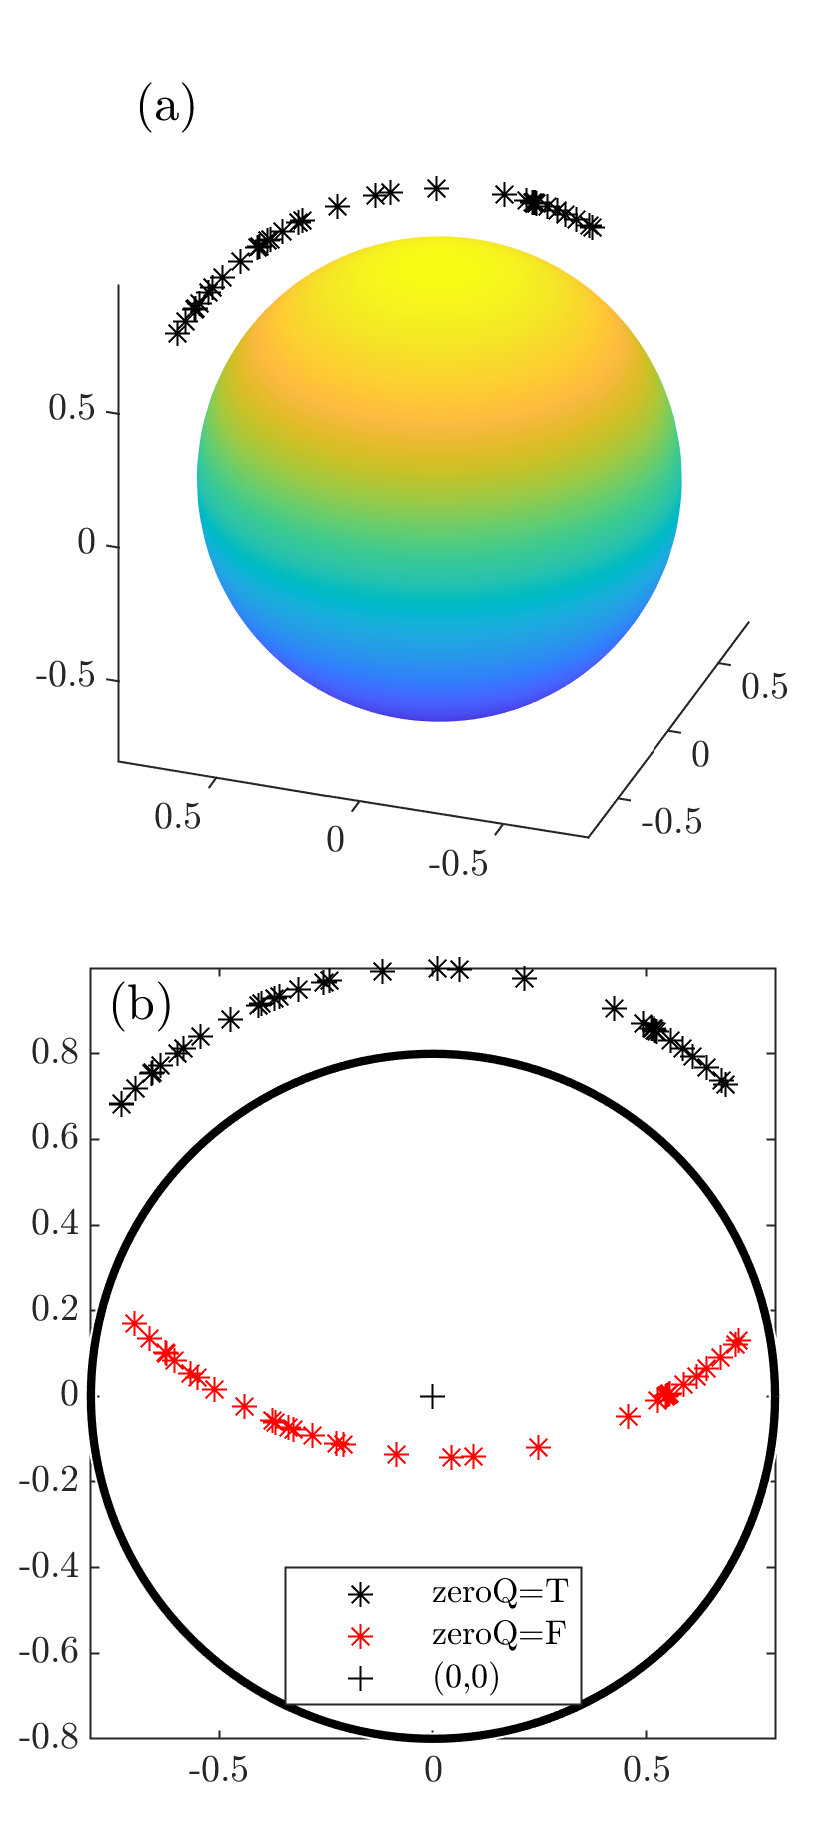
\includegraphics[scale=1]{bary-remove-deg.png}
	\caption{3D Cartesian to 2D Cartesian analogue of 8D Cartesian to 7D Cartesian degeneracy removal via rigid \gls{svd} transformation as used in barycentric interpolation approach. (a) Starting spherical arc points on surface of 2-sphere, (b) rotational symmetrization applied w.r.t. z-axis (analogous to U(1) symmetrization), and (c) degenerate dimension removed via \glsxtrlong{svd} transformation to 2D Cartesian with either the origin (black plus) preserved (black asterisks, \matlab{zeroQ=T}) for triangulation or ignored (red asterisks, \matlab{zeroQ=F}) for mesh intersection. The spheres (a,b) and circle (c) each have a radius of 0.8 and are used as a visualization aid only.}
	\label{fig:bary-remove-deg}
\end{figure*}

\begin{figure*}
	\centering
	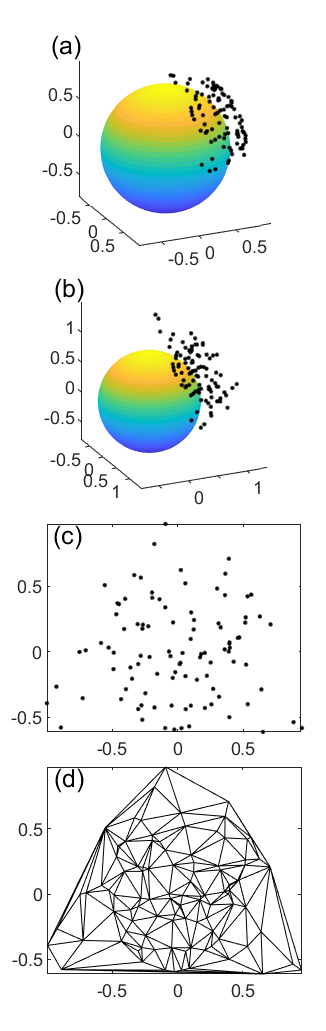
\includegraphics[scale=1]{bary-delaunay.png}
	\caption{3D Cartesian to 2D Cartesian analogue of 7D Cartesian to 6D Cartesian mesh triangulation used in barycentric interpolation approach. (a) 3D Cartesian \inpt{} points are (b) linearly projected onto hyperplane that is tangent to mean of starting points. (c) The degenerate dimension is removed via a rigid \gls{svd} transformation to 2D Cartesian and the Delaunay triangulation (black lines) is calculated, with \inpt{} vertices (red). Delaunay triangulation superimposed onto normalized \inpt{} points (d). The spheres in (a), (b), and (d) have a radius of 0.8 and are used for visualization only.}
	\label{fig:bary-delaunay}
\end{figure*}

While lower dimensional analogues are useful for visualizing and understanding the process of triangulation, a written description is also given in the following sections. As appropriate, we refer back to the teaching figures described in this section.

\subsubsection{\glsentrytitlecase{svd}{long} Transformation from 8D Cartesian to 7D Cartesian}
\label{sec:app:bary:tri:svd1}
To reduce the computational complexity of triangulating a high-dimensional mesh \cite{barberQuickhullAlgorithmConvex1996}, some simplifications are made. First, the degenerate \gls{gbo} dimension obtained from analytically minimizing $U(1)$ symmetry \cite{francisGeodesicOctonionMetric2019} is removed via a rigid (i.e. distance- and angle-preserving) \gls{svd} transformation,
%to enable use of MATLAB's quickhull \cite{barberQuickhullAlgorithmConvex1996} implementations such as \matlab{delaunayn} and \matlab{convhulln}. Removal of the degenerate dimension is done via a rigid \gls{svd} transformation,
analogous to a Cartesian rotation and translation (see 3D to 2D \gls{svd} transformation from \cref{fig:bary-remove-deg}b to \cref{fig:bary-remove-deg}c).
%Thus, a set of \glspl{gbo} originally represented by 8D Cartesian coordinates are collapsed to a 7D Cartesian representation while preserving both distances and angles among the points

\subsubsection{Linearly Project onto Hyperplane}
\label{sec:app:bary:tri:project}
Next, the resulting 7D Cartesian representation of each \gls{vfzgbo} is projected onto a hyperplane that is tangent to the centroid (i.e. mean) of the \gls{vfzgbo} set\footnote{This is \textit{not} a rigid transformation; however, it approximates one with sufficient accuracy to produce a high-quality triangulation in a \gls{vfz}.} (\cref{fig:bary-delaunay}a). By performing this linear projection, one of the dimensions becomes degenerate.

\subsubsection{\glsentrytitlecase{svd}{long} Transformation from 7D Cartesian to 6D Cartesian}
\label{sec:app:bary:tri:svd2}
This additional degeneracy is removed via a second \gls{svd} transformation, this time to 6D Cartesian coordinates (see 3D to 2D projection in \cref{fig:bary-delaunay}a-b). Finally, the resulting points can be triangulated via the quickhull algorithm \cite{barberQuickhullAlgorithmConvex1996} (see \vfzorepo{} function \matlab{sphconvhulln.m} and built-in MATLAB function \matlab{delaunayn()}), which relies on Euclidean distances\footnote{While the triangulation algorithm used in this work relies on Euclidean distances (the use of which is possible via the \gls{vfz} framework), other distance metrics that are non-Euclidean \cite{morawiecDistancesGrainInterfaces2019} could potentially be incorporated into the barycentric approach such as by doing an edge-length based simplex reconstruction \cite{connorHighdimensionalSimplexesSupermetric2017,boissonnatOnlyDistancesAre2017} using the \gls{vfz} triangulation edge lengths.}. Because the simplicial mesh is defined by a list of edges between vertices for each simplicial facet, this list applies immediately to the \gls{vfzgbo} set in its 7D Cartesian coordinates (i.e. no reverse transformation is necessary to use the mesh on the 6-sphere in 7D).

\subsection{Intersections in a \glsentrytitlecase{vfz}{long} Mesh}
\label{sec:app:bary:int}

Once the triangulation has been determined, we need to find which facet each \outpt{} point intersects (i.e. find the intersecting facet). There are two sub-steps:
\begin{itemize}
	\item[2.1] applying the same rigid transformation to the \outpt{} points as was applied to the \inpt{} points (otherwise the \outpt{} points won't line up properly with the mesh) (\cref{sec:app:bary:int:out-svd})
	\item[2.2] identifying facets nearby a \outpt{} point and testing for intersection (\cref{sec:app:bary:int:facets}).
\end{itemize}
\subsubsection{Apply Same \glsentrytitlecase{svd}{long} to Input and Prediction Points}
\label{sec:app:bary:int:out-svd}
The positions of the \outpt{} points need to be fixed relative to the mesh even after the rigid \gls{svd} transformation. %Thus, it is crucial to perform the same rigid \gls{svd} transformation (i.e. same rotation and translation) on the \outpt{} points as was applied to the \inpt{} points.
This is accomplished by:
\begin{itemize}
	\item[2.1a] concatenating both \inpt{} and
	\outpt{} points
	\item[2.1b] using the \matlab{interp5DOF.m} sub-routine \matlab{proj\_down.m} (which depends on MATLAB's built-in \gls{svd} implementation \matlab{svd()}) to perform the transformation
	\item[2.1c] subsequently separating the transformed \inpt{} and \outpt{} points (reverse of concatenation step)
\end{itemize}

To map new points onto the mesh, the \matlab{usv} structure output from \matlab{proj\_down.m} needs to be stored and supplied in future calls to \matlab{proj\_down.m}. Likewise, \matlab{usv} need to be supplied to \matlab{proj\_up.m} to perform the reverse \gls{svd} transformation.

\subsubsection{Testing Nearby Facets for Intersections}
\label{sec:app:bary:int:facets}
Once the \outpt{} points are lined up properly with the mesh, the facet containing the \outpt{} point (i.e. intersecting facet) is found. We define the intersecting facet as the one for which a point's barycentric coordinates are positive within a given tolerance. Consequently, we determine facet affiliation by:
\begin{enumerate}
	\item[2.2a] linearly projecting the \outpt{} point onto the hyperplane defined by a mesh facet's vertices (\cref{fig:bary-interp})
	\item[2.2b] computing the point's barycentric coordinates within the facet \cite{anatoliyCheckIfRay2015,skalaRobustBarycentricCoordinates2013} (see \vfzorepo{} function \matlab{projray2hypersphere.m})
	\item[2.2c] testing that all coordinates are positive \cite{langerSphericalBarycentricCoordinates2006} within a tolerance\footnote{Two tolerances are used: one for the initial computation of barycentric coordinates by projecting onto the hypersphere to determine facet affiliation (\matlab{projtol=1e-4}) and a larger tolerance (\matlab{inttol=1e-2}) for computation of barycentric coordinates to determine interpolated values (\cref{sec:app:bary-interp}). }
	\item[2.2d] repeating steps 2.2a-2.2c until an intersection is found or a stop condition is reached (see \matlab{nnMax} below).
\end{enumerate}

\begin{figure}
	\centering
	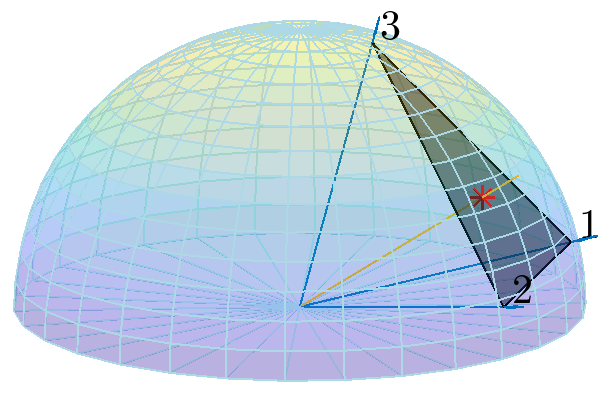
\includegraphics[scale=1]{bary-interp.png}
	\caption{A ray (red line) is linearly projected from the 2-sphere onto the hyperplane of a mesh facet (transparent black), shown as a red asterisk. The barycentric coordinates are computed as $\lambda_{i \in [1,3]} = \frac{1}{3}$. Because all barycentric coordinates are positive, it is determined that the projected point is an intersection with the mesh. Given vertex values of \num{8.183}, \num{3.446}, and \num{3.188} for vertices 1, 2, and 3, respectively, the interpolated value is calculated as \num{4.94} via \cref{eq:bary-interp}.}
	\label{fig:bary-interp}
\end{figure}

For further information on barycentric coordinates and its applications and generalizations, see \cite{anisimovSubdividingBarycentricCoordinates2016,budninskiyPowerCoordinatesGeometric2016,dyerBarycentricCoordinateNeighbourhoods2016,floaterGeneralizedBarycentricCoordinates2015,floaterInjectivityWachspressMean2010,hormannDiscretizingWachspressKernels2017,hormannMaximumEntropyCoordinates2008,langerHigherOrderBarycentric2008,langerSphericalBarycentricCoordinates2006,leiNewCoordinateSystem2020,meyerGeneralizedBarycentricCoordinates2002,peixotoVectorFieldReconstructions2014,pihajokiBarycentricInterpolationRiemannian2019,rustamovBarycentricCoordinatesSurfaces2010,skalaRobustBarycentricCoordinates2013,taoFastNumericalSolver2019,warrenBarycentricCoordinatesConvex2007}.

Due to the large number of facets per point of a high-dimensional triangulation (approximately \num{2000} facets per vertex for a \num{50000} point \gls{vfz} triangulation, or \num{1e8} total facets), some simplifications are made in order to determine intersections of \outpt{} points with the mesh. If every edge length of every facet were equal, only facets connected to the first \gls{nn} would need to be considered to find a proper intersection. However, since the \glspl{vfzgbo} are randomly sampled, edge lengths of facets are non-uniform, and non-unity aspect-ratio facets exist (\cref{fig:bary-delaunay}, \cref{fig:high-aspect-non-int}). If the facets have high-aspect ratios, the intersecting facets of \outpt{} points can be far from the \glspl{nn} mesh points relative to the \outpt{} points (see \cref{fig:high-aspect-non-int} inset), especially near the perimeter of a hyperspherical surface mesh. Rather than loop through every facet to find an intersection ($\sim$\num{1e8} facets in a \num{50000} \gls{vfzgbo} mesh), the \outpt{} point intersections are calculated by considering facets connected to up to some number of \gls{nn} mesh vertices (\matlab{nnMax}) relative to each \outpt{} point (in this work, \matlab{nnMax=10}). The \gls{nn} mesh vertices relative to a \outpt{} point are computed via the MATLAB built-in function \matlab{dsearchn} as in the \gls{nn} approach (\cref{sec:methods:interp:nn}). The facet IDs of facets connected to these \glspl{nn} are computed by calling built-in MATLAB function \matlab{find()}, as in \matlab{find(K==nn)}, where \matlab{K} is the triangulation from \vfzorepo{} function \matlab{sphconvhulln.m} and \matlab{nn} is the ID of one of the \gls{nn} mesh vertices. 

Some \outpt{} points will have no intersecting facet found.
%(which can occur just outside the piece-wise linear perimeter of the mesh due to finite resolution)
From our numerical testing, we determine that this non-intersection phenomenon occurs in two situations:
\begin{itemize}
	\item high-aspect ratio facets (described above)
	\item \outpt{} points that are positioned just outside the bounds of the mesh but within the bounds of the \gls{vfz}, due to the fact that the mesh is a piecewise linear approximation of a surface with a curved perimeter and that randomly sampled points typically do not fall on the true perimeter
\end{itemize}
In the first case, barycentric interpolation within high-aspect ratio facets may actually lead to worse interpolation error than a \gls{nn} interpolation strategy due to influence by \glspl{gb} far from the \outpt{} point. In the second case, there is no true intersection between the \outpt{} point and the mesh. Both issues can be addressed with the same strategy: we apply a \gls{nn} approach (\cref{sec:methods:interp:nn}) when an intersecting facet is not found within \matlab{nnMax} \glspl{nn}. In numerical tests, \gls{vfz} meshes composed of \num{388} and \num{50000} vertices produced non-intersection rates of \SI{12.07 \pm 1.02}{\percent} and \SI{0.68 \pm 0.11}{\percent}, respectively, over approximately \num{10} trials and using \num{10000} \outpt{} points for each trial.

Testing intersections for nearby facets is handled in the \vfzorepo{} function \matlab{intersect\_facet.m} and depends on the barycentric coordinate computations in \matlab{projray2hypersphere.m}.

\subsection{Interpolation via Barycentric Coordinates}
\label{sec:app:bary-interp}

Once a mesh triangulation has been determined (\cref{sec:app:bary:tri}), barycentric coordinates are recomputed for a \outpt{} point within the \inpt{} mesh (\cref{sec:app:bary:int}) using a somewhat larger tolerance; the interpolated value is found by taking the dot product of the \outpt{} point's barycentric coordinates and the properties of the corresponding vertices of the intersecting facet via
\begin{equation}
	\label{eq:bary-interp}
	v_{m,q}=\underset{i=1}{\overset{N}{\sum }}\lambda _{m,i} v_{m,i}
\end{equation}
where $\lambda_{m,i}$, $v_{m,q}$, $v_{m,i}$ and $N$, are the barycentric coordinates of the m-th \outpt{} point, interpolated property at the m-th \outpt{} point, property of the $i$-th vertex of the intersecting facet for the m-th \outpt{} point, and number of vertices in a given facet ($N = 7$ for facets of the simplicial mesh on the degeneracy-free 6-sphere), respectively. Interpolation of many \outpt{} points simultaneously can be accomplished by a simple, vectorized approach via MATLAB built-in function \matlab{dot()} as used in \vfzorepo{} function \matlab{interp\_bary\_fast.m}. This function assumes triangulation and weights have been precomputed. In other words, both \inpt{} and \outpt{} coordinates remain fixed, and only \inpt{} property values change. If this is the case, barycentric interpolation of new points is incredibly fast. By contrast, if \inpt{} coordinates change, the triangulation must be recomputed, and if \outpt{} coordinates change, the intersecting facets must be recomputed. Both triangulation and finding intersecting facets are computationally demanding with respect to memory and runtime (\cref{sec:results:efficiency}).